\section{Zielsetzung}
\label{sec:Zielsetzung}
Im folgenden Versuch wird die Ablenkung eines Elektronenstrahls unter dem Einfluss von
elektrischen und magnetischen Feldern untersucht.

\section{Theorie}
\label{sec:Theorie}
\subsection{Aufbau einer Kathodenstrahlröhre}
Zur Erzeugung eines Elektronenstrahls wird im Versuch eine sogenannte Kathodenstrahlröhre verwendet,
welche in Abbildung 1 schematisch dargestellt ist. Diese besteht im wesentlichen aus einer 
"Elektronenkanone", einem Ablenk- und einem Nachweissystem.
\begin{figure}[H]
  \centering
  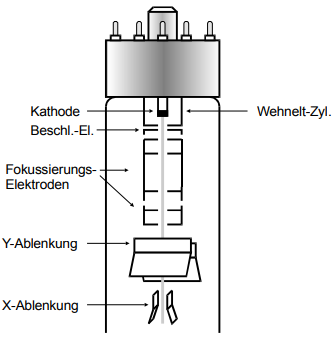
\includegraphics[height=7cm]{schema1.png}
  \caption{Schematischer Aufbau einer Kathodenstrahlröhre. \cite[S.2]{kent}}
\end{figure}
Aufgrund der Wechselwirkung von Luftmolekülen mit Elektronen wird der Versuch in einem Hochvakuum durchgeführt.
Durch Glühemission mittels indirekter Heizung werden aus einer zylindrischen Kathode, dessen Oberfläche aus einem Material
mit niedriger Elektronenaustrittsarbeit besteht, freie Elektronen erzeugt. Die Kathode ist
von einem zylindrischen Hohlkörper mit negativem Potential, dem Wehnelt-Zylinder, umgeben, 
der eine Bohrung in Strahlrichtung besitzt, mit dem man die Intensität des Elektronenstrahls
steuern kann. Die Elektrode vor dem Wehnelt-Zylinder besitzt ein hohes positives Potential $U_\text{B}$ 
(Beschleunigungsspannung), welches die Elektronen, die die Bohrung des Wehnelt-Zylinders passieren, 
beschleunigt. Aus der Energieerhaltung folgt somit
\begin{align}
\frac{m_\text{0} v_\text{z}^{2}}{2} = e_\text{0} U_\text{B},
\end{align}
mit der Elementarladung $e_\text{0}$, der Elektronenmasse $m_\text{0}$ und die Geschwindigkeit
$v_\text{z}$. \\~\\
Mithilfe der Elektroden vor der Beschleunigungselektrode wird der divergente Elektronenstrahl 
durch inhomogene E-Felder fokussiert. Die Brechkraft dieser Elektronenlinse lässt sich mithilfe 
der Spannung $U_\text{C}$ variieren. Trifft der Elektronenstrahl auf den leitenden Leuchtschirm, so werden
Störstellen im Kristallgitter des Schirms zur Emission von Lichtquanten angeregt. Davor besteht durch
zwei Plattenpaare, zwischen denen, mittels angelegten Spannungen $U_\text{d}$, elektrische Felder entstehen,
 die Möglichkeit, den Elektronenstrahl horizontal (in x-Richtung) und vertikal (in y-Richtung) abzulenken.

 \subsection{Ablenkung eines Elektronenstrahls im elektrischen Feld}
Passiert ein Elektron ein homogenes elektrisches Feld, so wirkt auf dieses eine Kraft $F$, die die
Flugbahn abhängig von der Feldstärke und der Elektronengeschwindigkeit verändert. 
Der Zusammenhang zwischen der Verschiebung $D$ des Leuchtfleckes auf dem Schirm und der
Ablenkspannung $U_\text{d}$ wird in Abbildung 2 verdeutlicht.
\begin{figure}[H]
  \centering
  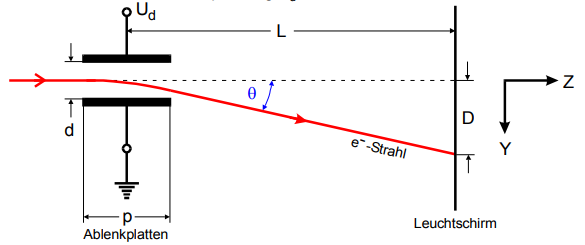
\includegraphics[height=5cm]{ablenkung1.png}
  \caption{Elektronenstrahlablenkung im elektrischen Feld. \cite[S.3]{kent}}
\end{figure}
Mit einem gegen die Plattenlänge $p$ kleinen Plattenabstand $d$ kann das Feld als homogen angesehen
werden und es gilt für die Kraft
\begin{align}
F = e_\text{0} \cdot E = e_\text{0} \frac{U_\text{d}}{d}.
\end{align}
Die Verschiebung D ergibt sich über die Komponentenbetrachtung der Geschwindigkeiten und Betrachtung
vom Winkel der Richtungsänderung $\theta$ und der Länge des Strahlwegs $L$  zu
\begin{align}
D = L \theta = \frac{p L U_\text{d}}{2 d U_\text{B}} \propto U_\text{d}.
\end{align}

\subsection{Erweiterung der Kathodenstrahlröhre zu einem
Kathodenstrahloszillographen}
Soll die Zeitabhängigkeit einer angelegten Wechselspannung dargestellt werden, so wird an das
Plattenpaar, das den Strahl in x-Richtung (horizontal) ablenkt, eine Sägezahnspannung angelegt.
Die zu untersuchende Spannung wird an die vertikal ablenken Platten angelegt.
Für die richtige Darstellung müssen Sägezahn- und Wechselspannungsfrequenz ($\nu_\text{S}$ und $\nu_\text{W}$) in einem geeigneten
Verhältnis zueinander stehen:
\begin{align}
n \nu_\text{S} = m \nu_\text{W} ; n, m \in ℕ.
\end{align}

\subsection{Ablenkung eines Elektronenstrahls im magnetischen Feld}
Bewegt sich ein Elektron mit der Ladung $q$ und der Geschwindigkeit $v$ durch ein magnetisches Feld $B$, so
wirkt auf dieses die Lorentzkraft
\begin{align}
F_\text{L} = q \vec{v} \times \vec{B},
\end{align}
welche nur auftritt, wenn die Geschwindigkeit eine Komponente senkrecht zum Magnetfeld besitzt.
Sie bewirkt also, dass sich das Elektron nun auf einer gektrümmten Bahn bewegt (Abbildung 3).
Der Krümmungsradius $r$ dieser Bahn ergibt sich, wenn die Zentrifugalkraft der Lorentzkraft gleichgesetzt
wird, wobei durch den Erhalt der kinetischen Energie $v_\text{0} = |\vec{v}|$ gelten muss:
\begin{align}
r = \frac{m_\text{0} v_\text{0}}{e_\text{0}B}.
\end{align}
\\~\\
\begin{figure}
  \centering
  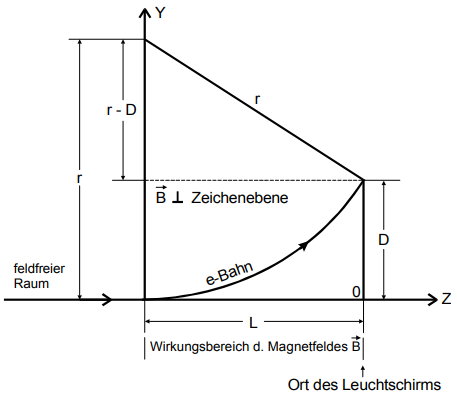
\includegraphics[height=7cm]{ablenkung2.png}
  \caption{Elektronenstrahlablenkung im magnetischen Feld und Beziehung zwischen L, D und r. \cite[S.2]{kent2}}
\end{figure}
In Abbildung 3 ist der Zusammenhang zwischen dem Krümmungsradius der Bahn und der Abweichung
vom Auftreffpunkt ohne Magnetfeld $D$ und der Länge des Einflussbereiches des Magnetfeldes $L$
dargestellt.
Mithilfe der Geschwindigkeit des Elektrons 
\begin{align*}
v_\text{0} = \sqrt{2U_\text{B} e_\text{0} / m_\text{0}}\;,
\end{align*} die abhängig von der Beschleunigungsspannung $U_\text{B}$ ist, und Gleichung (6)
lässt sich die spezifische Elektronenladung
\begin{align}
e_\text{0} = \frac{8 U_\text{B} D^{2} m_\text{0}}{(L^{2} + D^{2})B^{2}}
\end{align}
bestimmen.